\title{Syntax and Semantics Exam}
\author{
        Benjamin Bennetzen \\
        Student ID: 20204861 \\
        Computer Science, 4th semester\\
}
\date{\today}

\documentclass[12pt]{article}

\usepackage{tikz}
\usepackage{listings}
\usepackage{mathpartir}
\usepackage{ebproof}
\usepackage{amsmath}
\usepackage[utf8]{inputenc}
\usepackage{amssymb}
\usepackage{graphicx}
\usepackage{stmaryrd}

\newcommand{\R}{\mathbb{R}}
\newcommand{\F}{\mathbb{F}}
\newcommand{\num}[1]{\mathcal{N}\llbracket #1 \rrbracket}
\newcommand{\ul}[1]{\underline{#1}}

\begin{document}
\maketitle

\section{Exercise}
\subsection{}
Accepted words: 10, 01. Rejected words: 1, 0.

\subsection{}
$(01)^*|(10)^*$

\subsection{}
\begin{center}
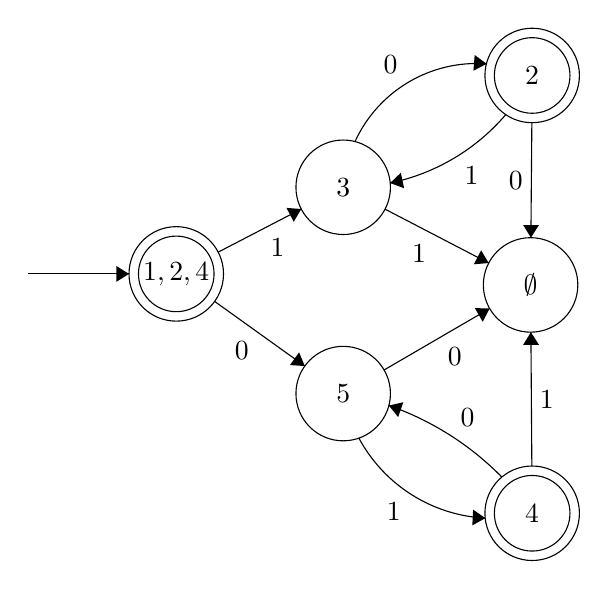
\begin{tikzpicture}[scale=0.2]
\tikzstyle{every node}+=[inner sep=0pt]
\draw [black] (24.1,-19.5) circle (3);
\draw (24.1,-19.5) node {${1,2,4}$};
\draw [black] (24.1,-19.5) circle (2.4);
\draw [black] (34.7,-14) circle (3);
\draw (34.7,-14) node {${3}$};
\draw [black] (34.7,-27.1) circle (3);
\draw (34.7,-27.1) node {${5}$};
\draw [black] (46.6,-20.2) circle (3);
\draw (46.6,-20.2) node {$\emptyset$};
\draw [black] (46.7,-6.9) circle (3);
\draw (46.7,-6.9) node {${2}$};
\draw [black] (46.7,-6.9) circle (2.4);
\draw [black] (46.7,-34.7) circle (3);
\draw (46.7,-34.7) node {${4}$};
\draw [black] (46.7,-34.7) circle (2.4);
\draw [black] (14.7,-19.5) -- (21.1,-19.5);
\fill [black] (21.1,-19.5) -- (20.3,-19) -- (20.3,-20);
\draw [black] (26.76,-18.12) -- (32.04,-15.38);
\fill [black] (32.04,-15.38) -- (31.1,-15.31) -- (31.56,-16.19);
\draw (30.53,-17.25) node [below] {$1$};
\draw [black] (26.54,-21.25) -- (32.26,-25.35);
\fill [black] (32.26,-25.35) -- (31.9,-24.48) -- (31.32,-25.29);
\draw (28.26,-23.8) node [below] {$0$};
\draw [black] (37.36,-15.39) -- (43.94,-18.81);
\fill [black] (43.94,-18.81) -- (43.46,-18) -- (43,-18.89);
\draw (39.52,-17.6) node [below] {$1$};
\draw [black] (35.444,-11.11) arc (155.45788:85.76489:8.505);
\fill [black] (43.81,-6.16) -- (43.05,-5.6) -- (42.97,-6.6);
\draw (37.71,-6.82) node [above] {$0$};
\draw [black] (37.3,-25.6) -- (44,-21.7);
\fill [black] (44,-21.7) -- (43.06,-21.67) -- (43.56,-22.54);
\draw (41.78,-24.15) node [below] {$0$};
\draw [black] (43.728,-35.009) arc (-92.94123:-151.75366:9.687);
\fill [black] (43.73,-35.01) -- (42.95,-34.47) -- (42.9,-35.47);
\draw (37.91,-34.02) node [below] {$1$};
\draw [black] (45.027,-9.382) arc (-40.49653:-78.2807:13.181);
\fill [black] (37.68,-13.73) -- (38.57,-14.06) -- (38.36,-13.08);
\draw (42.85,-12.67) node [below] {$1$};
\draw [black] (46.68,-9.9) -- (46.62,-17.2);
\fill [black] (46.62,-17.2) -- (47.13,-16.4) -- (46.13,-16.4);
\draw (46.14,-13.55) node [left] {$0$};
\draw [black] (37.6,-27.857) arc (70.77866:44.52645:18.704);
\fill [black] (37.6,-27.86) -- (38.19,-28.59) -- (38.52,-27.65);
\draw (42.59,-29.22) node [above] {$0$};
\draw [black] (46.68,-31.7) -- (46.62,-23.2);
\fill [black] (46.62,-23.2) -- (46.13,-24) -- (47.13,-24);
\draw (47.16,-27.45) node [right] {$1$};
\end{tikzpicture}
\end{center}

\section{Exercise}
\subsection{}
\begin{align*}
        S &\Rightarrow b \\
        S &\Rightarrow aSS \Rightarrow abS \Rightarrow abb \\
        S &\Rightarrow aSS \Rightarrow aaSSS \Rightarrow aabSS \Rightarrow aabbS \Rightarrow aabbb \\
\end{align*}

\subsection{}


\subsection{}
\begin{center}
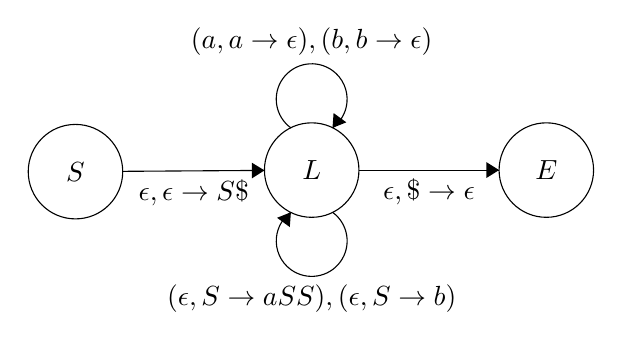
\begin{tikzpicture}[scale=0.2]
\tikzstyle{every node}+=[inner sep=0pt]
\draw [black] (21.1,-22.4) circle (3);
\draw (21.1,-22.4) node {$S$};
\draw [black] (36.1,-22.3) circle (3);
\draw (36.1,-22.3) node {$L$};
\draw [black] (51,-22.3) circle (3);
\draw (51,-22.3) node {$E$};
\draw [black] (24.1,-22.38) -- (33.1,-22.32);
\fill [black] (33.1,-22.32) -- (32.3,-21.83) -- (32.3,-22.83);
\draw (28.61,-22.89) node [below] {$\epsilon,\epsilon\rightarrow S\$$};
\draw [black] (39.1,-22.3) -- (48,-22.3);
\fill [black] (48,-22.3) -- (47.2,-21.8) -- (47.2,-22.8);
\draw (43.55,-22.8) node [below] {$\epsilon,\$\rightarrow \epsilon$};
\draw [black] (37.423,-24.98) arc (54:-234:2.25);
\draw (36.1,-29.55) node [below] {$(\epsilon,S\rightarrow aSS),(\epsilon,S\rightarrow b)$};
\fill [black] (34.78,-24.98) -- (33.9,-25.33) -- (34.71,-25.92);
\draw [black] (34.777,-19.62) arc (234:-54:2.25);
\draw (36.1,-15.05) node [above] {$(a,a\rightarrow \epsilon),(b,b\rightarrow \epsilon)$};
\fill [black] (37.42,-19.62) -- (38.3,-19.27) -- (37.49,-18.68);
\end{tikzpicture}
\end{center}

\section{Exercise}
For context-free languages the following holds. For any word $w$, where $\mid w \mid \geq p$ the following conditions will be satisfied.

\begin{itemize}
        \item for all $i \geq 0, uvxyz \in L$
        \item $|vy| > 0$
        \item $|vxy| \leq p$
\end{itemize}

We assume that L' is context-free and choose the word $a^pb^{p+1}c^{p+2}$ which is in L' and is clearly longer than $p$.

\section{Exercise}
\subsection{}
\begin{prooftree}
        \infer0[by rule 0]{\underline{0} \rightarrow 0}
        \infer1[$k = 2^{|0|} + 0$, by rule 3]{\underline{10} \rightarrow 2}
        \infer1[$k = 2^{|10|} + 2$, by rule 3]{\underline{110} \rightarrow 6}
\end{prooftree}

\subsection{}
First we create the base cases for \ul{1}, \ul{2}, and \ul{3}.

\begin{equation}
        [r_0] \quad \frac{}{\ul{0} \rightarrow 0}, \quad
        [r_1] \quad \frac{}{\ul{1} \rightarrow 1}, \quad
        [r_2] \quad \frac{}{\ul{1} \rightarrow 2}
\end{equation}

Now for the rest.

\begin{equation}
        [r_3] \quad \frac{w \rightarrow k'}{\ul{0}w \rightarrow k} \quad k = k'
\end{equation}

\begin{equation}
        [r_4] \quad \frac{w \rightarrow k'}{\ul{1}w \rightarrow k} \quad k = 3^{|w|} + k'
\end{equation}

\begin{equation}
        [r_5] \quad \frac{w \rightarrow k'}{\ul{2}w \rightarrow k} \quad k = 2 \cdot 3^{|w|} + k'
\end{equation}

\section{Exercise}
3, 6, 5

\end{document}
